\documentclass[a4paper]{easychair}

\usepackage[utf8]{inputenc}
\usepackage[french]{babel}
\usepackage{todonotes}

\newcommand\arr{\ocamlf{arr}}
\newcommand\arri[1]{\ocamlf{arr[}#1\ocamlf{]}}
\newcommand\eqdef{\overset{\text{def}}{=}}

\begin{document}

\title{Rapport de stage\\\large{Combinatoire et jonglerie musicale}}
\titlerunning{}
\author{Josué Moreau}
\institute{M1 MPRI, Université Paris-Saclay}
\authorrunning{}
\institute{}
\maketitle

\begin{abstract}
  Faut-il un abstract ???
\end{abstract}

\section{Introduction}
% contexte
La jonglerie a pour principe consiste à effectuer de manière continue des
lancers et rattrapés de balles dans les airs. Dans sa forme artistique, le
jongleur s'intéresse aux figures qu'il jongle afin de rendre sa performance la
plus esthétique possible. La jonglerie musicale, quant-à-elle s'intéresse aux
musiques qu'il est possible de jongler avec des balles qui jouent des sons lors
de certaines actions. Dans ce stage et dans la suite de ce rapport, nous nous
intéresserons uniquement aux balles qui jouent une note de musique lorsqu'elle
est rattrapée. Le jongleur souhaitant jouer une musique particulière lorsqu'il
jongle avec de telles balles doit donc les lancer de manière à ce qu'elles
retombent dans le bon ordre pour restituer la musique. Cet exercice est
difficile car l'ordre de lancer des balles associées aux notes n'est pas
nécessairement celui de la musique. De plus, la séquence de lancers à effectuer
pour jouer une musique donnée n'est généralement pas unique et n'existe pas
nécessairement. Enfin, même lorsqu'il existe une séquence de lancers à effectuer
pour restituer une musique, elle peut ne pas être jouable en pratique par le
jongleur pour différentes raisons pratiques. Dans ce stage, nous nous
intéresserons donc aux questions suivantes : Qu'est ce qui rend une séquence de
lancers jouable par un jongleur ? Étant donné une musique, existe-il une
séquence de lancers jouable qui restitue cette musique ?

% stage
Ce stage a été effectué en binôme, avec Léo Kulinski, également étudiant au M1
MPRI, et sous la direction de Florent Hivert et Nicolas Thiéry. Il s'est déroulé
au Laboratoire Interdisciplinaire des Sciences du Numérique et majoritairement
en distanciel. Durant ce stage, nous avons pu collaborer avec un jongleur
professionnel, Vincent de Lavenère, qui s'intéresse depuis de nombreuses années
à l'élaboration de spectacles de jonglerie musicale et qui a pu nous fournir de
nombreux éléments concrets concernant la pratique de la jonglerie.

% état de l'art
La jonglerie non musicale est un domaine qui a déjà été étudié à plusieurs
reprises, notamment par Claude Shannon~\cite{shannon}, ainsi que par Burkard
Polster~\cite{polster}. Notre modélisation de la jonglerie s'appuiera
principalement sur celle présente dans le livre de Burkard
Polster~\cite{polster}. Nous modifierons cette modélisation afin de correspondre
à la jonglerie musicale. À notre connaissance, il n'existe aucun article ou
ouvrage traitant de ce sujet.

\section{Formalisation mathématique de la jonglerie}
\subsection{Jonglerie à une main}
Dans un premier temps, on s'intéresse à la jonglerie à une main. Formellement,
une figure de jonglerie à une main est définie par une séquence de lancers. Un
lancer est paramétré par deux choses : l'instant auquel il est effectué et la
durée de vol de la balle lancée. Il est possible de ne pas spécifier le temps
auquel la balle est lancée si on considère que le premier lancer de la séquence
est effectué au temps $0$ et que par la suite chaque élément de la séquence est
effectué au temps suivant le lancer de son élément précédent. On peut voir sur
la figure~\ref{fig1} la séquence de jonglerie $3, 3, 3, 3, ...$. Lorsqu'il y a
un $0$ dans la séquence de jonglerie, on considère qu'il n'y a aucun lancer,
ainsi la séquence $4, 2, 0, 4, 2, 0, ...$ est représentée dans la figure 2.

\begin{figure}[!h]
  \centering
  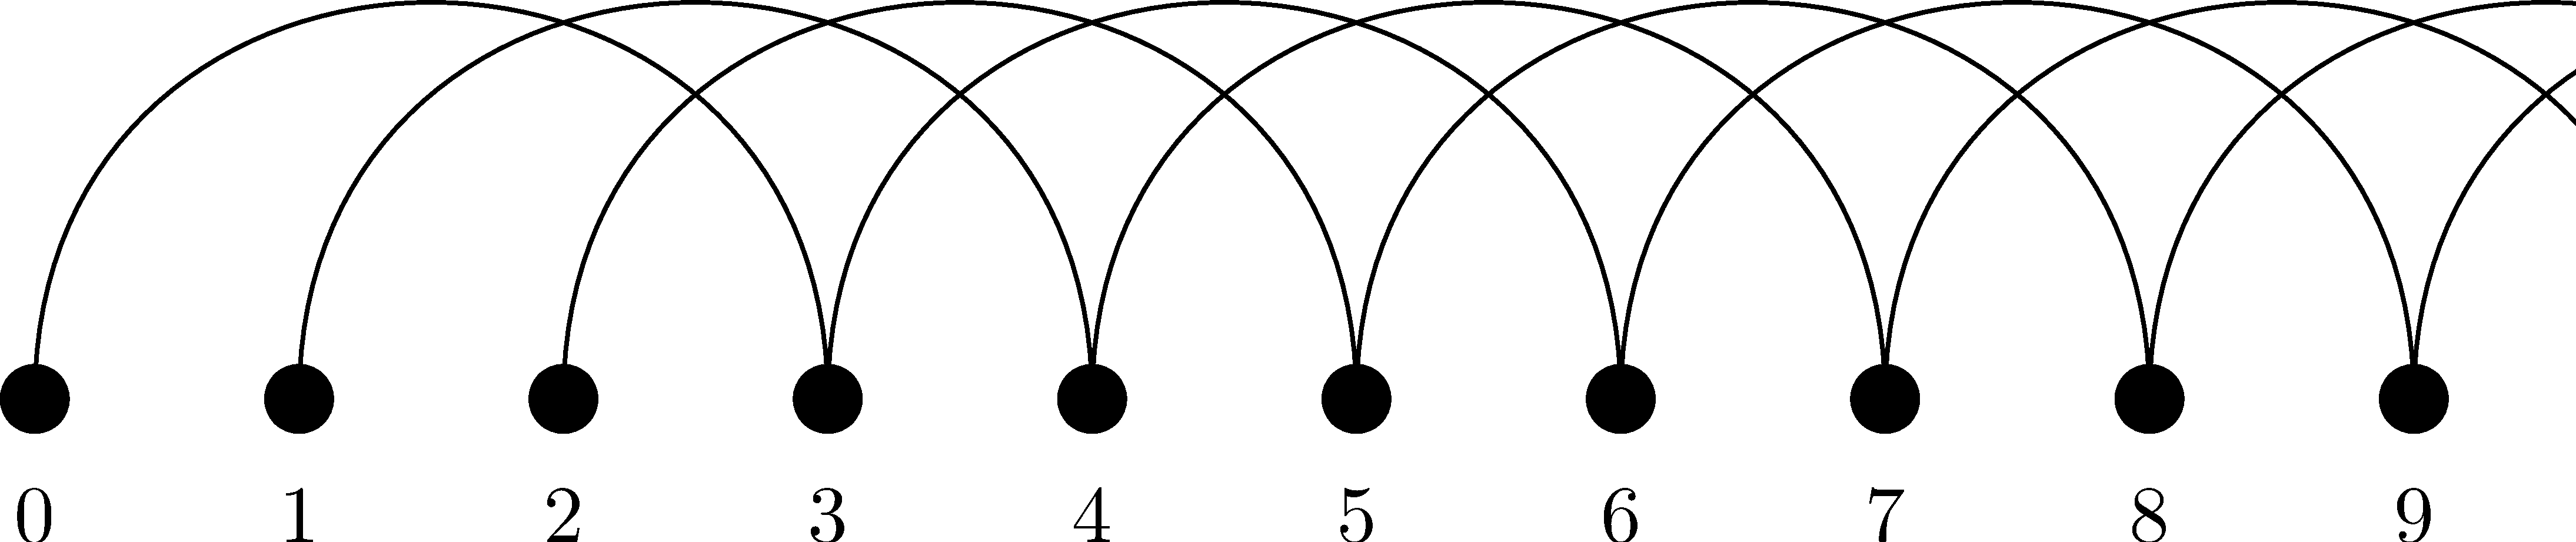
\includegraphics{figure-0}

  \caption{Séquence de jonglerie 3, 3, 3, 3, ...}
  \label{fig1}
\end{figure}

\begin{figure}[!h]
  \centering
  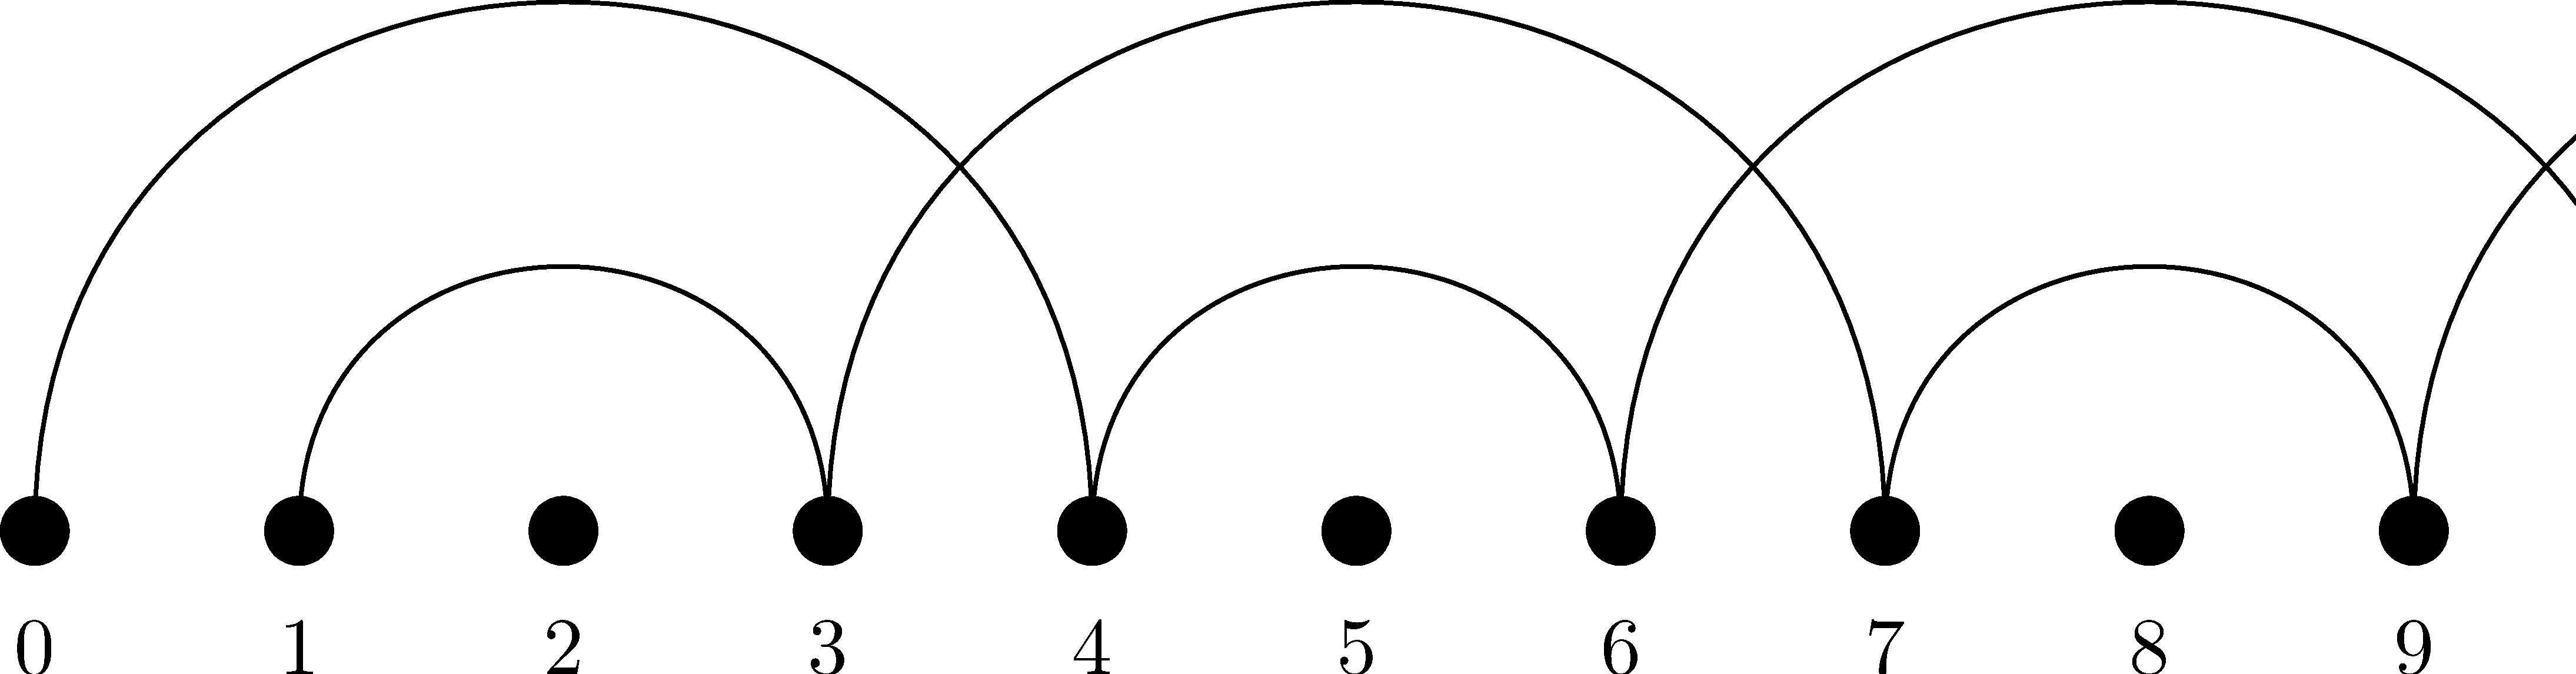
\includegraphics{figure-1}

  \caption{Séquence de jonglerie 4, 2, 0, 4, 2, 0, ...}
  \label{fig2}
\end{figure}


% présenter le "hand swap"

\section{Automates et jonglerie musicale}

\section{L'algorithme de composition}
\subsection{Pré-traitement}
\subsection{Le problème Exact Cover}
\subsection{Résolution avec MILP}
\subsection{Résolution avec Dancing Links}

\section{Perspectives et travaux futurs}

\section{Conclusion}
\label{sec:conclusion}

\bibliographystyle{plain}
\bibliography{./biblio}

\end{document}

% LocalWords:  Cover distanciel binôme
